\section{Heuristica de busqueda local}

Para encontrar soluciones aproximadas al problema de optimizar una funci\'on $f:S \rightarrow \mathbb{R}$ definida sobre un conjunto $S$ de instancias, la heur\'istica de b\'usqueda local consiste en tomar un elemento $e \in S$ y buscar entre los elementos ``cercanos'' a $e$ uno $e'$ en el cual el valor que toma la funci\'on sea mejor ($f(e') < f(e)$ \'o $f(e') > f(e)$ dependiendo de si se busca m\'inimo a o m\'aximo).
El concepto de cercan\'ia o vecidad se puede definir seg\'un cualquier criterio que se crea conveniente de forma tal que evaluar la vecindad sea barato. Se busca en lo posible que las vecindades de cada punto sean peque\~nas para que se pueda encontrar r\'apidamente un vecino mejor en caso de que exista.
La heur\'istica itera el procedimiento de optimizaci\'on local creando una sucesi\'on de soluciones aproximadas $(X_0, X_1, ... , X_m)$ en $S$ donde el elemento $X_m$ tiene la propiedad de ser un extremo local de la funci\'on $f$ seg\'un el criterio definido de vecindad.

\subsection{Criterios de vecindad}
Para el problema enunciado del TP, el conjunto $S$ es el conjunto de caminos entre el nodo de partida y el de llegada. Debido a que las $w_1$ y $w_2$ son funciones no negativas, el camino acotado de costo m\'inimo estar\'a en $S' \subseteq S$, el subconjunto de todos los caminos simples. Por lo tanto solo se considerar\'a $S'$ como conjunto de instancias.

Establecemos la siguiente notaci\'on: $C = (v_1, ..., v_m)$ ser\'a un camino y $A_c$ el conjunto de aristas que lo conforman. Dos caminos $C = (v_1, ... , v_n)$ y $C' = (v'_1, ... , v'_m)$ en $S'$ son vecinos $C \sim C'$ en su vecindad $N_j$ correspondiente si se cumple su condicion asociada.\\

Definiremos a continuacion varias vecindades:
\begin{enumerate}
    \item $ N_1(C): \exists v \notin C \mid A_{c'} = A_c - \{(v_i,v_{i+1}),(v_{i+1},v_{i+2})\} + \{(v_i,v),(v,v_{i+2})\}$\\
    	Este criterio consiste en reemplazar un nodo intermedio en una tripla, tal que las sumas de los costos $w_2$ de las nuevas aristas sea menor que los costos de las aristas que existian originalmente, teniendo en cuenta tambien, que la mejora no implique que los nuevos costos $w_1$ sobrepasen la cota $K \in \mathbb{R}_{>0}$ establecida en el problema.
    \item $ N_2(C): \exists v \notin C \mid A_{c'} = A_c - \{(v_i,v_{i+1})\} + \{(v_i,v),(v,v_{i+1})\}$\\
    	Este criterio consiste en la inserci\'on de un nodo $v$ adyacente en comun a $v_i$ y $v_{i+1}$ entre ellos, de forma tal que disminuya el costo $w_2$ en el sendero entre $v_i$ $\rightarrow$ $v_{i+1}$ pero que nuevamente no se sobrepase la cota sobre $w_1$ establecida para el problema.
    \item $ N_3(C):  A_{c'} = A_c - \{(v_i,v_{i+1}), (v_{i+1},v_{i+2})\} + \{(v_i,v_{i+2})\}$\\
    	Este criterio consiste en la eliminaci\'on de un nodo intermedio entre una tripla consecutiva de nodos, siendo reemplazado por una arista existente en el grafo que conecte directamente los nodos $v_i$ $\rightarrow$ $v_{i+1}$, de forma tal que la contracci\'on del sendero entre $v_i$ $\rightarrow$ $v_{i+1}$ disminuya el costo $w_2$ pero tampoco sobrepase la cota sobre $w_1$ estipulada en el problema.
    \item $N(C): N_1 \cup N_2 \cup N_3$\\
    	Se trata de la union de todos los criterios anteriores, una exploracion completa de esta vecindad en una iteraci\'on consiste en buscar las mejores modificaciones de las vecindades previas y la aplicacion de la mejor de ellas sobre la solucion actual de dicha iteracion.
\end{enumerate}

\textbf{Nota:} $C = C'$ se considera que son caminos vecinos en todas las vecindades. Adem\'as de los criterios de cada vecindad, debe valer, que el nuevo camino resultante $C'$ sea factible, es decir, respete la cota de $w_1$ de $K$ luego de ser modificado.

\begin{figure}[H]
\centering
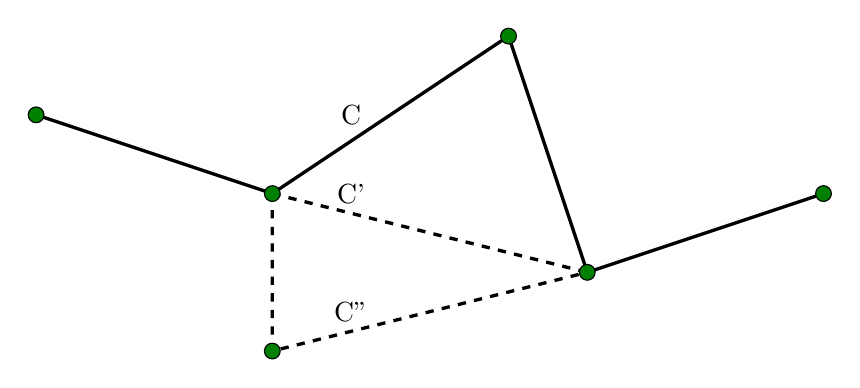
\begin{tikzpicture}

\draw[black, solid, very thick] (-1,2) -- (2,1) -- (5,3) -- (6,0) -- (9,1);
\draw[black, dashed, very thick] (2,1) -- (6,0);
\draw[black, dashed, very thick] (2,1) -- (2,-1)  -- (6,0);
\filldraw[fill=green!50!black, draw=black] (2,-1) circle [radius=1mm];
\filldraw[fill=green!50!black, draw=black] (-1,2) circle [radius=1mm];
\filldraw[fill=green!50!black, draw=black] (2,1) circle [radius=1mm];
\filldraw[fill=green!50!black, draw=black] (5,3) circle [radius=1mm];
\filldraw[fill=green!50!black, draw=black] (6,0) circle [radius=1mm];
\filldraw[fill=green!50!black, draw=black] (9,1) circle [radius=1mm];
\node(c) at (3,2) {C};
\node(c') at (3,1) {C'};
\node(c'') at (3,-0.5) {C''};

\end{tikzpicture}
\caption{Tres caminos vecinos entre si.}
\end{figure}

\subsection{Explicacion detallada del algoritmo propuesto}
Sea $s$ una solucion factible, es decir, un camino entre $u,v$ tal que el costo del camino $w_1 \leq K$,
para plantear esta heur\'istica definimos $N(s) = \{ $ conjunto de soluciones vecinas de s$\}$ = $\{$ caminos entre u,v tal que $w_1 \leq K$ y difieren en solo un nodo de $s\}$.\\

Se plantearon 3 posibles enfoques para aplicar busqueda local sobre esta vecindad, a continuacion se explicar\'an cada uno.

\subsubsection{Obtencion de la solucion inicial factible}

Para obtener la solucion inicial factible de nuestra heur\'istica ejecutamos el algoritmo de camino m\'inimo de Dijkstra, entre los nodos u y v, minimizando la funcion $w_1$, acto seguido validamos si $dist(w_1, src, dst) > K$ entonces no existe soluci\'on factible, caso contrario tenemos una soluci\'on factible inicial para comenzar las 
iteraciones de busqueda local.

\subsubsection{Criterio de terminaci\'on}
El criterio de terminacion fue repetir las iteraciones sobre las nuevas soluciones que se iban obteniendo, hasta que no se obtiene mejora.
Pueden aplicarse las iteraciones con exploraciones sobre las vecindades $N_1$, $N_2$, $N_3$ por separado o bien combinarse en $N$ como mencionamos anteriormente. Esto se selecciona mediante un parametro en el metodo main del codigo de la busqueda local.

\subsubsection{Pseudocodigo}

A continuaci\'on el pseudoc\'odigo de la b\'usqueda local.
\begin{algorithmic}

 \Procedure{$Bq\_Local$}{$Grafo\: g, \:vertice\: v_1,\: vertice \: v_2, \: int \: k, tipo\_busqueda$}{$\rightarrow lista<eje>\: camino$}

 \State $lista<eje> \: camino\: =\: dijkstra(g, \:v_1,\: v_2, \:costoW1)$
 \If{camino.costoW1 $>$ K}
 \State No existe solucion.
 \EndIf
 \State  $bool\: valor\_mejora\: = \:\infty$

 \While{$valor\_mejora > 0$}

  \State $switch(tipo\_busqueda)$
	\State$\: \: \: 	case\: subdividirPares$
		\State$\: \: \: \: \: 	\:valor\_mejora\: = \: bqLocalEntrePares(g,camino)$
	\State$	\: \: \: case\: contraerTriplas$		
		\State$\: \: \: \: \: 	\:valor\_mejora\: = \: bqLocalContraerTriplas(g,camino)$
	\State$	\: \: \: case \:mejorarTriplas:		$
		\State$\: \: \: \: \: 	\:valor\_mejora\: = \: bqlocalEntreTriplasReemplazando(g,camino)$
	\State$	\: \: \: case \:combinarVecindades:		$
		\State$\: \: \: \: \: 	\:valor\_mejora\_1\: = \: estimar\_bqLocalEntrePares(g,camino)$
		\State$\: \: \: \: \: 	\:valor\_mejora\_2\: = \: estimar\_bqLocalContraerTriplas(g,camino)$
		\State$\: \: \: \: \: 	\:valor\_mejora\_3\: = \: estimar\_bqlocalEntreTriplasReemplazando(g,camino)$
		\State$\: \: \: \: \: 	\:valor\_mejora\: = \: Aplicar$ $la$ $mejor$ $de$ $las$ $3$ $vecindades$ $exploradas$ $o$ $setear$ $valor\_mejora$ $en$ $0$ $indicando$ $que$ $no$ $se$ $pudo$ $mejorar$ $mas$.


\EndWhile

 \State $return \:camino$

 \EndProcedure

\end{algorithmic}

A continuac\'ion se explicar\'an las vecindades definidas al comienzo de esta secci\'on.

\subsubsection{Reemplazar un nodo intermedio en una 3-upla consecutiva de nodos del camino}
Si el camino tiene longuitud 2, es decir hay una arista directa entre $u,v$ , no hay nada que hacer en este caso, caso contrario, sea $S = \{u,...,v_l, v_{l+1}, v_{l+2}, v_{l+3} ..., v\}$ la solucion actual. Lo que hace en este caso es iterar sobre todas las 3-uplas consecutivas del camino, en este ejemplo sea $(vl, v_{l+1}, v_{l+2})$ una 3-upla, $(v_{l+1}, v_{l+2}, v_{l+3})$ la siguiente a iterar, etc...\\ \\
Para cada 3-upla iterada se revisan los vecinos en comun entre los extremos de la 3-upla buscando una mejor conexi\'on entre extremos reemplazando el nodo intermedio, es decir, se busca una nueva conexion entre los extremos tal que, si el nuevo nodo intermedio es $v_t$, vale que:
\begin{itemize}
	\item Mejore la conexion de la 3-upla respecto a $w_2$, $w_2(vl, v_{t}) + w_2(vt, v_{l+2}) < w_2(vl, v_{l+1}) + w_2(v_{l+1}, v_{l+2})$
	\item Este cambio, reflejado en la nueva solucion candidata S', no sobrepase la cota K establecida sobre $w_1$, es decir, sea factible.
\end{itemize}


Una iteracion consiste en recorrer todas las 3-uplas del camino obteniendo de los vecinos en com\'un de los extremos de cada 3-upla, si es posible, la mejor forma de mejorar esta conexion, ademas recordando la mejor 3-upla para aplicar la mejora a lo largo de la iteraci\'on, tal que el camino resultante de aplicar esta mejora sea el minimo sobre $w_2$ en la vecindad $N_1(s)$. Mas formalmente, se busca una solucion vecina del camino S, tal que siendo $w_1(P), w_2(P)$ los costos sobre $w_1$ y $w_2$ respectivamente de una solucion, y $S' = S \setminus \{(v_k, v_{k+1}); (v_{k+1}, v_{k+2})\} \cup \{(v_k, v_t);(v_t, v_{k+2})\}$ la nueva solucion obtenida, entonces valga que:
\begin{itemize}
	\item Sea factible, pertenezca a $N_1(S)$, $ w_1(S') \leq K$
	\item Sea minima respecto de $w_2$ en la vecindad $N(S)$, $w_2(S') \leq w_2(T)$ $ \forall$ $ T \in N(S) $
\end{itemize}

\subsubsection{Insertar un nodo intermedio en un par consecutivo de nodos del camino}
Este enfoque es basicamente igual al anterior, solo que en lugar de iterar sobre 3-uplas reemplazando el nodo intermedio, se itera sobre pares consecutivos de nodos de la solucion S $(v_k, v_{k+1})$ buscando si existe, un vecino en comun entre los extremos tal que el sendero $(v_k, v_t, v_{k+1})$ tenga costo menor(de forma minima entre los vecinos) sobre $w_2$ que la arista directa y que reflejado en la solucion candidata S' que surge de aplicar este cambio, siga siengo factible($w_2(S') \leq K$). La iteracion de sigue siendo sobre toda la vecindad $N_2(S)$ y quedandose con el mejor $S' \in N_2(S)$ posible.


\subsubsection{Contracci\'on de 3-uplas}

Similar a los casos anteriores, itera sobre las 3-uplas de nodos del camino, intentando eliminar el nodo intermedio y buscar una arista que conecte directamente los nodos de los extremos. Sean los 3 nodos $v_1$, $v_2$ y $v_3$, y el subcamino de aristas formado por ellos $[ (v_1, v_2), (v_2, v_3)]$, se encontrar la arista $(v_1, v_3)$, tal que:

\begin{itemize}
	\item $costoW2((v_1, v_3)) \leq costoW2((v_1, v_2)) + costoW2((v_2, v_3))$
	\item Que el camino, eliminando el nodo $v_2$ y las aristass $(v_1, v_2), (v_2, v_3)$ y conectando los nodos $v_1$ y $v_3$ mediante la arista directa $(v_1, v_3)$ siga sin sobrepasar la cota K establecida sobre $w_1$, es decir, sea factible.
\end{itemize}

\subsection{Nivel de optimalidad de las soluciones}
\subsubsection{Familias de grafos malas para esta heur\'istica}

La heur\'istica va a fallar en todos los casos en los cuales no se pueda mejorar un par o tripla de nodos agregando, quitando o reemplazando de a un nodo, por ejemplo, casos en los que la mejora sea un subcamino de longitud mayor a 2, o casos en los que el camino \'optimo no tiene ning\'in tipo de conexi\'on con el camino m\'inimo seg\'un $w_1$. Podria intentar arreglarse el problema generalizando la idea de contraer triplas a contraer subcaminos consecutivos de mayor longuitud con alguna variaci\'on de BFS pero podr\'ia incrementarse mucho el cardinal de las vecindades, siendo esto un problema para la exploraci\'on de las mismas.

En el proximo ejemplo. Mostraremos un grafo en el cual la heur\'istica no devuelve la soluci\'on \'optima.

\begin{figure}[H]
	\centering
	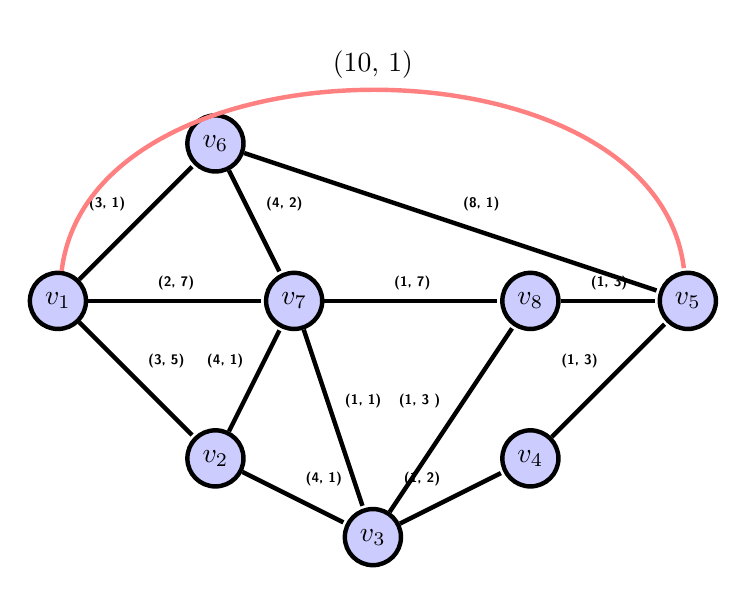
\begin{tikzpicture}[shorten >=1pt, auto, node distance=3cm, ultra thick,
   edge_style/.style={draw=black, ultra thick,font=\sffamily\tiny\bfseries}]
	\node [circle,draw=black,fill=blue!20] (n1) at (1,2)  {$v_1$};
	\node [circle,draw=black,fill=blue!20] (n6) at (3,4)  {$v_6$};
	\node [circle,draw=black,fill=blue!20] (n2) at (3,0)  {$v_2$};
	\node [circle,draw=black,fill=blue!20] (n7) at (4,2)  {$v_7$};
	\node [circle,draw=black,fill=blue!20] (n3) at (5,-1)  {$v_3$};
	\node [circle,draw=black,fill=blue!20] (n4) at (7,0)  {$v_4$};
	\node [circle,draw=black,fill=blue!20] (n8) at (7,2)  {$v_8$};
	\node [circle,draw=black,fill=blue!20] (n5) at (9,2)  {$v_5$};

	\foreach \from/\to/\distance/\cost in {
		n1/n6/3/1,
		n1/n7/2/7,
		n1/n2/3/5,
		n6/n7/4/2,
		n2/n7/4/1,
		n6/n5/8/1,
		n2/n3/4/1,
		n3/n4/1/2,
		n4/n5/1/3,
		n7/n8/1/7,
		n8/n5/1/3,
		n7/n3/1/1,
		n3/n8/1/3
		}
	  \draw [edge_style] (\from) edge node{(\distance, \cost)} (\to);
	
	\path (n1) edge [bend left=83, draw=red!50] node{(10, 1)} (n5);

	\end{tikzpicture}
	\caption{Ejemplo grafo malo para la heur\'istica.} \label{fig:vida_real_1}
\end{figure}

Para esta entrada, la soluci\'on inicial factible que nos brinda el algoritmo de dijkstra comienza siendo:\\
\textbf{Nota: } Los pesos entre corchetes representan a $w_1$ y $w_2$ respectivamente.
\begin{lstlisting}[frame=single]
	Camino inicial: (1)----[2, 7]---->(7)----[1, 7]---->(8)----[1, 3]---->(5)
\end{lstlisting}

La cual no tiene ninguna relaci\'on con la soluci\'on \'optima. La b\'usqueda local finaliza devolviendo un camino:
\begin{lstlisting}[frame=single]
	(1)----[3, 1]---->(6)----[4, 2]---->(7)----[1, 1]---->(3)----[1, 2]---->(4)----[1, 3]---->(5)	
\end{lstlisting}

Veamos que no es el camino \'optimo:
Salida del algoritmo de soluci\'on exacta
\begin{lstlisting}[frame=single]
	10 1 2 1 5, es decir. La arista directa entre (1) y (5) con un peso w1: 10 y peso w2: 1
\end{lstlisting}

\subsection{Complejidad}
Para la explorac\'ion de las vecindades $N_1$ y $N_2$ se recorren las duplas/triplas consecutivas de nodos, segun corresponda, lo cual toma $O(n)$, y por cada una de las triplas, se obtienen los vecinos en comun de los nodos extremos, esto cuesta $O(n)$, sin embargo, fue mejorada la constante debido a un preprocesamiento mencionado debajo. Luego la complejidad temporal de explorar sucesivamente las vecindades mencionadas es $k*O(n^2)$, donde k es la cantidad de iteraciones necesarias hasta finalizar la b\'usqueda local.\\
Para la vecindad $N_3$ se recorren todas las triplas consecutivas, nuevamente con un costo temporal de \'orden lineal. Para cada tripla, se verifica en tiempo constante por matriz de adyacencia que exista una arista directa entre los extremos y se validan las restricciones de factibilidad y mejora de $w_1$ y $w_2$ respectivamente. Luego, el costo temporal de exploracion sucesiva se la vecindad es $k*O(n)$, donde k es la cantidad de iteraciones que fueron realizadas hasta finalizar la b\'usqueda local.\\

\textbf{Complejidad exploracion combinada:} En este caso la exploraci\'on completa de la vecindad $N$ consiste en una exploracion consecutiva de las vecindades $N_1, N_2, N_3$, con lo cual la complejidad de explorar toda la vecindad, es la suma de las complejidades de las vecindades que la componen, es decir $O(n) + O(n^2) + O(n^2) $ = $ O(n^2)$. Luego de la exploracion, en tiempo constante se obtiene la mejora factible que mas impacte en la minimizacion de $w_2$ y se la aplica en tiempo constante dado que el camino esta implementado con listas enlazadas, y poseemos el iterador al punto del camino a modificar, ya sea insertando o eliminando nodos. El costo temporal total de la b\'usqueda local combinada es $k*O(n^2)$ donde k es la cantidad de iteraciones que fueron necesarias hasta obtener el extremo local.\\

\textbf{Nota:} Se acotan por $O(n)$ los recorridos de triplas y duplas consecutivas, porque se mantiene siempre un camino \texttt{simple} y a lo sumo contiene a todos los nodos del grafo, es decir que el camino tiene longuitud n como m\'aximo. 

\subsection{Taboo list}
  Definimos una taboo list como una lista en la cual se encuentran los nodos que pertenecen al camino soluci\'on actual, de forma de evitar que la b\'usqueda local intente mejorar las conexiones utilizano nodos que ya pertenecen al camino.Esto es indispesable para evitar la generacion de ciclos en el caso de agregar un nodo al subdividir una arista o reemplazar un nodo
intermedio entre otros dos. Si se mantienen disjuntos disjuntos el conjunto de nodos del camino actual y los nodos restantes del grafo, cualquier eleccion que hagamos no generar\''a ciclos.

\vspace{2mm}

La taboo list est\'a implementada como un vector de bool que forma parte de los atributos de un camino del grafo, de forma de poder consultar la pertenencia de un nodo al camino en tiempo constante.

\vspace{2mm}

	Otra opcion considerada fue no restringir la b\'usqueda de nuevos nodos, pero luego deber\'ia realizarse una poda de ciclos del camino. En la muchos de los casos esto realizari\'ia una mejora importante del camino, pero esto aumenta la complejidad de la heur\'istica y deja de ser b\'usqueda local, dado que la soluci\'on que surja de la poda en muchos casos no va a estar en la vecindad del camino.
 
\subsection{Prec\'omputo de vecinos en comun}
Para agilizar la b\'usqueda de vecinos en comun entre 2 nodos para la exploracion de las vecindades y aprovechando que el grafo es estatico, es decir, no se agregan o quitan aristas luego de ser leido de la entrada, se precomputa, para cada par de nodos $v_i,v_j$ una lista con los nodos adyacentes en comun. Luego para obtener los vecinos en comun en los diversos algoritmos implementados, solo basta con obtener esta informaci\'on precomputada.

\subsection{Experimentacion: Mediciones de Performance}
En esta secci\'on se mostrar\'an resultados de complejidad temporal emp\'irica acerca del costo promedio de una iteracion de busqueda local, veremos que tal como analizamos en la secci\'on anterior de complejidad, dicho costo esta situacion en el orden cuadratico $O(n^2)$.
Para tener una mejor idea del comportamiento del algoritmo, realizamos pruebas sobre grafos aleatorios de distintos tama\~nos(en cantidad de nodos), y por cada cantidad $n$ de nodos, variamos las densidades de aristas dentro de cierto rango alrededor de una funcion de $n$, las densidades elegidas fueron:
\begin{itemize}
	\item m = $a*n + b$. Es decir una cantidad lineal de aristas en base a los nodos. $a \in \mathbb{N}_{>1}$
	\item m = $\frac{n*(n-1)}{2}$. Es decir grafos cercanos o iguales a cliques de n nodos.
\end{itemize}


\textbf{Nota: } Como mencionamos anteriormente, las funciones son variadas en un rango, es decir, por ejemplo, para el caso de cliques, los grafos generados tienen entre $\frac{n*(n-1)}{5}$ y $\frac{n*(n-1)}{2}$ aristas para aleatorizar mas la generacion de grafos densos.\\

\textbf{Nota: } Los graficos que contienen puntos rojos y una curva verde, indican, para cada valor del eje X(cantidad de nodos), los puntos rojos son los tiempos de ejecucion para los diferentes valores de aristas en el rango de la familia, asimismo, la curva verde indica el promedio de estos puntos para cada X. \\
\textbf{Nota: }Para verificar que se trata de una curva cuadratica dividimos las funciones por $n^1$, $n^2$, $n^3$, $n^4$ y como en los trabajos practicos anteriores concluimos de que curva se trata.\\

A continuacion presentamos los resultados de estos experimentos:\\
\subsubsection{Rendimiento para grafos con densidad lineal de aristas}
\begin{itemize}
	\item cant nodos min = $200$
	\item cant nodos max = $2000$
	\item peso maximo w1 = $200$
	\item peso maximo w2 = $200$
	\item step nodos = $200$
	\item step aristas = $2500$
	\item aristas minimas = $n-1$
	\item aristas maximas = $10*n$
\end{itemize}								

\begin{center}
	\textbf{Tiempo de ejecuci\'on en microsegundos para esta familia}\\
	\textbf{$y = f(x)$}\\
	\includegraphics[scale=0.7]{experimentos/bqlocal/rendimiento_aristas_lineales/complexity_variation.png}
\end{center}

\begin{center}
	\textbf{$y = f(x)/x$}\\
	\includegraphics[scale=0.7]{experimentos/bqlocal/rendimiento_aristas_lineales/complexity_med_over_n.png}
\end{center}

\begin{center}
	\textbf{$y = f(x)/x^2$}\\
	\includegraphics[scale=0.7]{experimentos/bqlocal/rendimiento_aristas_lineales/complexity_med_over_n_square.png}
\end{center}

\begin{center}
	\textbf{$y = f(x)/x^3$}\\
	\includegraphics[scale=0.7]{experimentos/bqlocal/rendimiento_aristas_lineales/complexity_med_over_n_cube.png}
\end{center}

\begin{center}
	\textbf{$y = f(x)/x^4$}\\
	\includegraphics[scale=0.7]{experimentos/bqlocal/rendimiento_aristas_lineales/complexity_med_over_n_fourth.png}
\end{center}

\subsubsection{Rendimiento para grafos con densidad cuadratica de aristas}
\begin{itemize}
	\item cant nodos min = $100$
	\item cant nodos max = $2000$
	\item peso maximo w1 = $200$
	\item peso maximo w2 = $200$
	\item step nodos = $200$
	\item step aristas = $2500$
	\item aristas minimas = $\frac{n*(n-1)}{17}$
	\item aristas maximas = $\frac{n*(n-1)}{14}$
\end{itemize}								

\begin{center}
	\textbf{Tiempo de ejecuci\'on en microsegundos para esta familia}\\
	\textbf{$y = f(x)$}\\
	\includegraphics[scale=0.7]{experimentos/bqlocal/rendimiento_aristas_cuadraticas_3/complexity_variation.png}
\end{center}

\begin{center}
	\textbf{$y = f(x)/x$}\\
	\includegraphics[scale=0.7]{experimentos/bqlocal/rendimiento_aristas_cuadraticas_3/complexity_med_over_n.png}
\end{center}

\begin{center}
	\textbf{$y = f(x)/x^2$}\\
	\includegraphics[scale=0.7]{experimentos/bqlocal/rendimiento_aristas_cuadraticas_3/complexity_med_over_n_square.png}
\end{center}

\begin{center}
	\textbf{$y = f(x)/x^3$}\\
	\includegraphics[scale=0.7]{experimentos/bqlocal/rendimiento_aristas_cuadraticas_3/complexity_med_over_n_cube.png}
\end{center}

\begin{center}
	\textbf{$y = f(x)/x^4$}\\
	\includegraphics[scale=0.7]{experimentos/bqlocal/rendimiento_aristas_cuadraticas_3/complexity_med_over_n_fourth.png}
\end{center}

Como vemos en las 2 secciones de resultados anteriores, para $n^2$, $n^3$ se mantiene constante dentro de un rango muy reducido en el eje Y, pero para $n^3$ y $n^4$ es una funcion marcadamente decreciente, con lo cual, llegamos a la conclusion de que la curva es cuadr\'atica, afirmando nuestra complejidad teorica esperada.


\subsection{Experimentacion: Variaci\'on evolutiva de mejora en cada iteracion}
\subsubsection{Rendimiento evolutivo en grafos muy densos}
Resumen del analisis:
\begin{itemize}
	\item Cantidad de tests realizados: 24
	\item Iteraciones promedio: 5
	\item Minima cantidad de iteraciones: 2
	\item Maxima cantidad de iteraciones: 16
\end{itemize}

\begin{center}
	\textbf{Ejemplo de la evoluci\'on en la mejora de la solucion durante las iteraciones de la busqueda local}\\
	\textbf{$y = f(x)$, para cada x=numero de iteracion, f(x) expresa la mejora obtenida en $w_2$ en dicha iteracion}\\
	\includegraphics[scale=0.7]{experimentos/bqlocal/rendimiento_evolucion_iteraciones_cliques/test-results/bqlocal/instancia_120_7130_in_iters.png}
\end{center}

En general, todas las funciones son estrictamente decrecientes, salvo excepciones donde en ciertos puntos crece muy poco y vuelve a decrecer mas fuertemente. Esto nos da la pauta de que el grado de mejora en cada iteracion durante la vida del ciclo de la busqueda local decrece a medida que hacemos mas iteraciones, para finalmente estancarse en cero y llegar al criterio de terminaci\'on.

\subsection{Experimentacion: Distintas soluciones iniciales factibles}
Como mencionamos antes, se utiliza Dijkstra sobre $w_1$ para obtener la solucion inicial factible, para comenzar las iteraciones de b\'usqueda local. En esta secci\'on decidimos variar esto y establecer la solucion inicial de busqueda local con la heuristica golosa. Para ciertos grafos preestablecidos que pueden encontrarse en la carpeta \texttt{grafos especiales} las soluciones finales de busqueda local con los 2 modos de solucion inicial son iguales, lo que vari\'o de forma notable fue la cantidad de iteraciones de busqueda local necesarias para llegar a dicha solucion final, debajo se muestra una tabla indicando esto:
\begin{center}
	\begin{tabular}{ | l | c | c |}
	  Grafo especial numero & Cant. iters Dijkstra & Cant. iters Greedy \\
	  \hline
	  Grafo\_1.txt & 3 & 0 \\
	  \hline
	  Grafo\_2.txt & 2 & 0 \\
	  \hline
	  Grafo\_3.txt & 1 & 0 \\
	  \hline
	  Grafo\_4.txt & 0 & 0 \\
	  \hline
	\end{tabular}
\end{center}

Asumimos que esto se debe a la calidad de la soluci\'on provista por el algoritmo goloso.